\documentclass[1p]{elsarticle_modified}
%\bibliographystyle{elsarticle-num}

%\usepackage[colorlinks]{hyperref}
%\usepackage{abbrmath_seonhwa} %\Abb, \Ascr, \Acal ,\Abf, \Afrak
\usepackage{amsfonts}
\usepackage{amssymb}
\usepackage{amsmath}
\usepackage{amsthm}
\usepackage{scalefnt}
\usepackage{amsbsy}
\usepackage{kotex}
\usepackage{caption}
\usepackage{subfig}
\usepackage{color}
\usepackage{graphicx}
\usepackage{xcolor} %% white, black, red, green, blue, cyan, magenta, yellow
\usepackage{float}
\usepackage{setspace}
\usepackage{hyperref}

\usepackage{tikz}
\usetikzlibrary{arrows}

\usepackage{multirow}
\usepackage{array} % fixed length table
\usepackage{hhline}

%%%%%%%%%%%%%%%%%%%%%
\makeatletter
\renewcommand*\env@matrix[1][\arraystretch]{%
	\edef\arraystretch{#1}%
	\hskip -\arraycolsep
	\let\@ifnextchar\new@ifnextchar
	\array{*\c@MaxMatrixCols c}}
\makeatother %https://tex.stackexchange.com/questions/14071/how-can-i-increase-the-line-spacing-in-a-matrix
%%%%%%%%%%%%%%%

\usepackage[normalem]{ulem}

\newcommand{\msout}[1]{\ifmmode\text{\sout{\ensuremath{#1}}}\else\sout{#1}\fi}
%SOURCE: \msout is \stkout macro in https://tex.stackexchange.com/questions/20609/strikeout-in-math-mode

\newcommand{\cancel}[1]{
	\ifmmode
	{\color{red}\msout{#1}}
	\else
	{\color{red}\sout{#1}}
	\fi
}

\newcommand{\add}[1]{
	{\color{blue}\uwave{#1}}
}

\newcommand{\replace}[2]{
	\ifmmode
	{\color{red}\msout{#1}}{\color{blue}\uwave{#2}}
	\else
	{\color{red}\sout{#1}}{\color{blue}\uwave{#2}}
	\fi
}

\newcommand{\Sol}{\mathcal{S}} %segment
\newcommand{\D}{D} %diagram
\newcommand{\A}{\mathcal{A}} %arc


%%%%%%%%%%%%%%%%%%%%%%%%%%%%%5 test

\def\sl{\operatorname{\textup{SL}}(2,\Cbb)}
\def\psl{\operatorname{\textup{PSL}}(2,\Cbb)}
\def\quan{\mkern 1mu \triangleright \mkern 1mu}

\theoremstyle{definition}
\newtheorem{thm}{Theorem}[section]
\newtheorem{prop}[thm]{Proposition}
\newtheorem{lem}[thm]{Lemma}
\newtheorem{ques}[thm]{Question}
\newtheorem{cor}[thm]{Corollary}
\newtheorem{defn}[thm]{Definition}
\newtheorem{exam}[thm]{Example}
\newtheorem{rmk}[thm]{Remark}
\newtheorem{alg}[thm]{Algorithm}

\newcommand{\I}{\sqrt{-1}}
\begin{document}

%\begin{frontmatter}
%
%\title{Boundary parabolic representations of knots up to 8 crossings}
%
%%% Group authors per affiliation:
%\author{Yunhi Cho} 
%\address{Department of Mathematics, University of Seoul, Seoul, Korea}
%\ead{yhcho@uos.ac.kr}
%
%
%\author{Seonhwa Kim} %\fnref{s_kim}}
%\address{Center for Geometry and Physics, Institute for Basic Science, Pohang, 37673, Korea}
%\ead{ryeona17@ibs.re.kr}
%
%\author{Hyuk Kim}
%\address{Department of Mathematical Sciences, Seoul National University, Seoul 08826, Korea}
%\ead{hyukkim@snu.ac.kr}
%
%\author{Seokbeom Yoon}
%\address{Department of Mathematical Sciences, Seoul National University, Seoul, 08826,  Korea}
%\ead{sbyoon15@snu.ac.kr}
%
%\begin{abstract}
%We find all boundary parabolic representation of knots up to 8 crossings.
%
%\end{abstract}
%\begin{keyword}
%    \MSC[2010] 57M25 
%\end{keyword}
%
%\end{frontmatter}

%\linenumbers
%\tableofcontents
%
\newcommand\colored[1]{\textcolor{white}{\rule[-0.35ex]{0.8em}{1.4ex}}\kern-0.8em\color{red} #1}%
%\newcommand\colored[1]{\textcolor{white}{ #1}\kern-2.17ex	\textcolor{white}{ #1}\kern-1.81ex	\textcolor{white}{ #1}\kern-2.15ex\color{red}#1	}

{\Large $\underline{12n_{0098}~(K12n_{0098})}$}

\setlength{\tabcolsep}{10pt}
\renewcommand{\arraystretch}{1.6}
\vspace{1cm}\begin{tabular}{m{100pt}>{\centering\arraybackslash}m{274pt}}
\multirow{5}{120pt}{
	\centering
	\includegraphics[width=112pt]{../../../GIT/diagram.site/Diagrams/png/2187_12n_0098.png}\\
\ \ \ A knot diagram\footnotemark}&
\allowdisplaybreaks
\textbf{Linearized knot diagam} \\
\cline{2-2}
 &
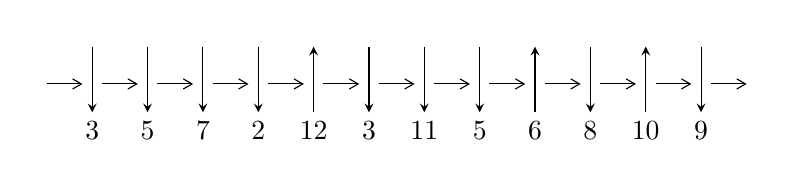
\begin{tikzpicture}[x=20pt, y=17pt]
	% nodes
	\node (C0) at (0, 0) {};
	\node (C1) at (1, 0) {};
	\node (C1U) at (1, +1) {};
	\node (C1D) at (1, -1) {3};

	\node (C2) at (2, 0) {};
	\node (C2U) at (2, +1) {};
	\node (C2D) at (2, -1) {5};

	\node (C3) at (3, 0) {};
	\node (C3U) at (3, +1) {};
	\node (C3D) at (3, -1) {7};

	\node (C4) at (4, 0) {};
	\node (C4U) at (4, +1) {};
	\node (C4D) at (4, -1) {2};

	\node (C5) at (5, 0) {};
	\node (C5U) at (5, +1) {};
	\node (C5D) at (5, -1) {12};

	\node (C6) at (6, 0) {};
	\node (C6U) at (6, +1) {};
	\node (C6D) at (6, -1) {3};

	\node (C7) at (7, 0) {};
	\node (C7U) at (7, +1) {};
	\node (C7D) at (7, -1) {11};

	\node (C8) at (8, 0) {};
	\node (C8U) at (8, +1) {};
	\node (C8D) at (8, -1) {5};

	\node (C9) at (9, 0) {};
	\node (C9U) at (9, +1) {};
	\node (C9D) at (9, -1) {6};

	\node (C10) at (10, 0) {};
	\node (C10U) at (10, +1) {};
	\node (C10D) at (10, -1) {8};

	\node (C11) at (11, 0) {};
	\node (C11U) at (11, +1) {};
	\node (C11D) at (11, -1) {10};

	\node (C12) at (12, 0) {};
	\node (C12U) at (12, +1) {};
	\node (C12D) at (12, -1) {9};
	\node (C13) at (13, 0) {};

	% arrows
	\draw[->,>={angle 60}]
	(C0) edge (C1) (C1) edge (C2) (C2) edge (C3) (C3) edge (C4) (C4) edge (C5) (C5) edge (C6) (C6) edge (C7) (C7) edge (C8) (C8) edge (C9) (C9) edge (C10) (C10) edge (C11) (C11) edge (C12) (C12) edge (C13) ;	\draw[->,>=stealth]
	(C1U) edge (C1D) (C2U) edge (C2D) (C3U) edge (C3D) (C4U) edge (C4D) (C5D) edge (C5U) (C6U) edge (C6D) (C7U) edge (C7D) (C8U) edge (C8D) (C9D) edge (C9U) (C10U) edge (C10D) (C11D) edge (C11U) (C12U) edge (C12D) ;
	\end{tikzpicture} \\
\hhline{~~} \\& 
\textbf{Solving Sequence} \\ \cline{2-2} 
 &
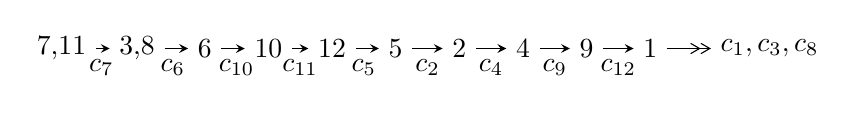
\begin{tikzpicture}[x=23pt, y=7pt]
	% node
	\node (A0) at (-1/8, 0) {7,11};
	\node (A1) at (17/16, 0) {3,8};
	\node (A2) at (17/8, 0) {6};
	\node (A3) at (25/8, 0) {10};
	\node (A4) at (33/8, 0) {12};
	\node (A5) at (41/8, 0) {5};
	\node (A6) at (49/8, 0) {2};
	\node (A7) at (57/8, 0) {4};
	\node (A8) at (65/8, 0) {9};
	\node (A9) at (73/8, 0) {1};
	\node (C1) at (1/2, -1) {$c_{7}$};
	\node (C2) at (13/8, -1) {$c_{6}$};
	\node (C3) at (21/8, -1) {$c_{10}$};
	\node (C4) at (29/8, -1) {$c_{11}$};
	\node (C5) at (37/8, -1) {$c_{5}$};
	\node (C6) at (45/8, -1) {$c_{2}$};
	\node (C7) at (53/8, -1) {$c_{4}$};
	\node (C8) at (61/8, -1) {$c_{9}$};
	\node (C9) at (69/8, -1) {$c_{12}$};
	\node (A10) at (11, 0) {$c_{1},c_{3},c_{8}$};

	% edge
	\draw[->,>=stealth]	
	(A0) edge (A1) (A1) edge (A2) (A2) edge (A3) (A3) edge (A4) (A4) edge (A5) (A5) edge (A6) (A6) edge (A7) (A7) edge (A8) (A8) edge (A9) ;
	\draw[->>,>={angle 60}]	
	(A9) edge (A10);
\end{tikzpicture} \\ 

\end{tabular} \\

\footnotetext{
The image of knot diagram is generated by the software ``\textbf{Draw programme}" developed by Andrew Bartholomew(\url{http://www.layer8.co.uk/maths/draw/index.htm\#Running-draw}), where we modified some parts for our purpose(\url{https://github.com/CATsTAILs/LinksPainter}).
}\phantom \\ \newline 
\centering \textbf{Ideals for irreducible components\footnotemark of $X_{\text{par}}$} 
 
\begin{align*}
I^u_{1}&=\langle 
4.18552\times10^{72} u^{61}+3.25275\times10^{72} u^{60}+\cdots+1.83626\times10^{74} b-1.12303\times10^{74},\\
\phantom{I^u_{1}}&\phantom{= \langle  }-1.03434\times10^{74} u^{61}-5.26235\times10^{74} u^{60}+\cdots+1.83626\times10^{74} a+1.05888\times10^{76},\\
\phantom{I^u_{1}}&\phantom{= \langle  }u^{62}+5 u^{61}+\cdots-113 u+1\rangle \\
I^u_{2}&=\langle 
b,\;- u^3+a+2,\;u^4+u^2- u+1\rangle \\
I^u_{3}&=\langle 
-120 a^2 u+44 a^2-865 a u+691 b+202 a+177 u-134,\;a^3- a^2 u+8 a^2-4 a u+a-5 u-7,\;u^2- u+1\rangle \\
I^u_{4}&=\langle 
b,\;- u^3- u^2+a-2 u-1,\;u^6+u^5+2 u^4+2 u^3+2 u^2+2 u+1\rangle \\
\\
\end{align*}
\raggedright * 4 irreducible components of $\dim_{\mathbb{C}}=0$, with total 78 representations.\\
\footnotetext{All coefficients of polynomials are rational numbers. But the coefficients are sometimes approximated in decimal forms when there is not enough margin.}
\newpage
\renewcommand{\arraystretch}{1}
\centering \section*{I. $I^u_{1}= \langle 4.19\times10^{72} u^{61}+3.25\times10^{72} u^{60}+\cdots+1.84\times10^{74} b-1.12\times10^{74},\;-1.03\times10^{74} u^{61}-5.26\times10^{74} u^{60}+\cdots+1.84\times10^{74} a+1.06\times10^{76},\;u^{62}+5 u^{61}+\cdots-113 u+1 \rangle$}
\flushleft \textbf{(i) Arc colorings}\\
\begin{tabular}{m{7pt} m{180pt} m{7pt} m{180pt} }
\flushright $a_{7}=$&$\begin{pmatrix}1\\0\end{pmatrix}$ \\
\flushright $a_{11}=$&$\begin{pmatrix}0\\u\end{pmatrix}$ \\
\flushright $a_{3}=$&$\begin{pmatrix}0.563286 u^{61}+2.86580 u^{60}+\cdots-4.40887 u-57.6652\\-0.0227937 u^{61}-0.0177140 u^{60}+\cdots-3.56182 u+0.611587\end{pmatrix}$ \\
\flushright $a_{8}=$&$\begin{pmatrix}1\\u^2\end{pmatrix}$ \\
\flushright $a_{6}=$&$\begin{pmatrix}-0.398010 u^{61}-2.06178 u^{60}+\cdots+15.0559 u+34.3666\\0.108322 u^{61}+0.265127 u^{60}+\cdots+7.66296 u-0.403405\end{pmatrix}$ \\
\flushright $a_{10}=$&$\begin{pmatrix}u\\u^3+u\end{pmatrix}$ \\
\flushright $a_{12}=$&$\begin{pmatrix}u^3\\u^5+u^3+u\end{pmatrix}$ \\
\flushright $a_{5}=$&$\begin{pmatrix}-0.364245 u^{61}-1.69585 u^{60}+\cdots-5.63070 u+34.5483\\-0.0484629 u^{61}-0.227602 u^{60}+\cdots+6.86074 u-0.394692\end{pmatrix}$ \\
\flushright $a_{2}=$&$\begin{pmatrix}0.351605 u^{61}+1.74250 u^{60}+\cdots-1.36842 u-32.2841\\0.0484629 u^{61}+0.227602 u^{60}+\cdots-6.86074 u+0.394692\end{pmatrix}$ \\
\flushright $a_{4}=$&$\begin{pmatrix}-0.586080 u^{61}-2.88351 u^{60}+\cdots+0.847056 u+58.2767\\0.0227937 u^{61}+0.0177140 u^{60}+\cdots+3.56182 u-0.611587\end{pmatrix}$ \\
\flushright $a_{9}=$&$\begin{pmatrix}-0.0628689 u^{61}-0.211226 u^{60}+\cdots+1.30026 u-10.6392\\-0.121039 u^{61}-0.637166 u^{60}+\cdots+18.6696 u-0.0518508\end{pmatrix}$ \\
\flushright $a_{1}=$&$\begin{pmatrix}0.0216935 u^{61}-0.0922332 u^{60}+\cdots+16.0468 u-1.14018\\0.115443 u^{61}+0.357638 u^{60}+\cdots+2.47253 u-0.00153419\end{pmatrix}$\\&\end{tabular}
\flushleft \textbf{(ii) Obstruction class $= -1$}\\~\\
\flushleft \textbf{(iii) Cusp Shapes $= 0.152156 u^{61}+1.18827 u^{60}+\cdots+7.99782 u-8.81670$}\\~\\
\newpage\renewcommand{\arraystretch}{1}
\flushleft \textbf{(iv) u-Polynomials at the component}\newline \\
\begin{tabular}{m{50pt}|m{274pt}}
Crossings & \hspace{64pt}u-Polynomials at each crossing \\
\hline $$\begin{aligned}c_{1}\end{aligned}$$&$\begin{aligned}
&u^{62}+71 u^{61}+\cdots+267 u+1
\end{aligned}$\\
\hline $$\begin{aligned}c_{2},c_{4}\end{aligned}$$&$\begin{aligned}
&u^{62}-13 u^{61}+\cdots+15 u-1
\end{aligned}$\\
\hline $$\begin{aligned}c_{3},c_{6}\end{aligned}$$&$\begin{aligned}
&u^{62}+3 u^{61}+\cdots-8192 u-1024
\end{aligned}$\\
\hline $$\begin{aligned}c_{5}\end{aligned}$$&$\begin{aligned}
&u^{62}+4 u^{61}+\cdots-10 u^2+1
\end{aligned}$\\
\hline $$\begin{aligned}c_{7},c_{10}\end{aligned}$$&$\begin{aligned}
&u^{62}-5 u^{61}+\cdots+113 u+1
\end{aligned}$\\
\hline $$\begin{aligned}c_{8}\end{aligned}$$&$\begin{aligned}
&u^{62}+4 u^{61}+\cdots-3025807 u+537503
\end{aligned}$\\
\hline $$\begin{aligned}c_{9}\end{aligned}$$&$\begin{aligned}
&u^{62}+44 u^{60}+\cdots+9664 u+824
\end{aligned}$\\
\hline $$\begin{aligned}c_{11}\end{aligned}$$&$\begin{aligned}
&u^{62}-21 u^{61}+\cdots+12769 u+1
\end{aligned}$\\
\hline $$\begin{aligned}c_{12}\end{aligned}$$&$\begin{aligned}
&u^{62}-6 u^{61}+\cdots-1248 u+64
\end{aligned}$\\
\hline
\end{tabular}\\~\\
\newpage\renewcommand{\arraystretch}{1}
\flushleft \textbf{(v) Riley Polynomials at the component}\newline \\
\begin{tabular}{m{50pt}|m{274pt}}
Crossings & \hspace{64pt}Riley Polynomials at each crossing \\
\hline $$\begin{aligned}c_{1}\end{aligned}$$&$\begin{aligned}
&y^{62}-147 y^{61}+\cdots-20183 y+1
\end{aligned}$\\
\hline $$\begin{aligned}c_{2},c_{4}\end{aligned}$$&$\begin{aligned}
&y^{62}-71 y^{61}+\cdots-267 y+1
\end{aligned}$\\
\hline $$\begin{aligned}c_{3},c_{6}\end{aligned}$$&$\begin{aligned}
&y^{62}-57 y^{61}+\cdots+9961472 y+1048576
\end{aligned}$\\
\hline $$\begin{aligned}c_{5}\end{aligned}$$&$\begin{aligned}
&y^{62}-4 y^{61}+\cdots-20 y+1
\end{aligned}$\\
\hline $$\begin{aligned}c_{7},c_{10}\end{aligned}$$&$\begin{aligned}
&y^{62}+21 y^{61}+\cdots-12769 y+1
\end{aligned}$\\
\hline $$\begin{aligned}c_{8}\end{aligned}$$&$\begin{aligned}
&y^{62}+16 y^{61}+\cdots-11200434939731 y+288909475009
\end{aligned}$\\
\hline $$\begin{aligned}c_{9}\end{aligned}$$&$\begin{aligned}
&y^{62}+88 y^{61}+\cdots+13013520 y+678976
\end{aligned}$\\
\hline $$\begin{aligned}c_{11}\end{aligned}$$&$\begin{aligned}
&y^{62}+45 y^{61}+\cdots-163345321 y+1
\end{aligned}$\\
\hline $$\begin{aligned}c_{12}\end{aligned}$$&$\begin{aligned}
&y^{62}-30 y^{61}+\cdots-185344 y+4096
\end{aligned}$\\
\hline
\end{tabular}\\~\\
\newpage\flushleft \textbf{(vi) Complex Volumes and Cusp Shapes}
$$\begin{array}{c|c|c}  
\text{Solutions to }I^u_{1}& \I (\text{vol} + \sqrt{-1}CS) & \text{Cusp shape}\\
 \hline 
\begin{aligned}
u &= -0.197990 + 0.977965 I \\
a &= -0.817839 - 0.403463 I \\
b &= -0.181458 + 0.756746 I\end{aligned}
 & \phantom{-}3.58947 - 0.62301 I & \phantom{-}3.36345 + 2.22600 I \\ \hline\begin{aligned}
u &= -0.197990 - 0.977965 I \\
a &= -0.817839 + 0.403463 I \\
b &= -0.181458 - 0.756746 I\end{aligned}
 & \phantom{-}3.58947 + 0.62301 I & \phantom{-}3.36345 - 2.22600 I \\ \hline\begin{aligned}
u &= \phantom{-}0.504265 + 0.860405 I \\
a &= \phantom{-}8.46750 - 1.97416 I \\
b &= \phantom{-}0.596380 - 0.013951 I\end{aligned}
 & -1.08843 - 2.05155 I & \phantom{-}143.754 + 62.581 I \\ \hline\begin{aligned}
u &= \phantom{-}0.504265 - 0.860405 I \\
a &= \phantom{-}8.46750 + 1.97416 I \\
b &= \phantom{-}0.596380 + 0.013951 I\end{aligned}
 & -1.08843 + 2.05155 I & \phantom{-}143.754 - 62.581 I \\ \hline\begin{aligned}
u &= \phantom{-}0.315979 + 0.963839 I \\
a &= \phantom{-}1.63289 + 2.55056 I \\
b &= \phantom{-}0.261416 - 0.638531 I\end{aligned}
 & -0.90689 - 2.60619 I & -4.21909 + 1.98730 I \\ \hline\begin{aligned}
u &= \phantom{-}0.315979 - 0.963839 I \\
a &= \phantom{-}1.63289 - 2.55056 I \\
b &= \phantom{-}0.261416 + 0.638531 I\end{aligned}
 & -0.90689 + 2.60619 I & -4.21909 - 1.98730 I \\ \hline\begin{aligned}
u &= -0.399423 + 0.961282 I \\
a &= -0.895928 + 0.237941 I \\
b &= \phantom{-}0.251217 + 1.010200 I\end{aligned}
 & \phantom{-}3.47148 - 0.76506 I & \phantom{-}5.05392 + 1.67806 I \\ \hline\begin{aligned}
u &= -0.399423 - 0.961282 I \\
a &= -0.895928 - 0.237941 I \\
b &= \phantom{-}0.251217 - 1.010200 I\end{aligned}
 & \phantom{-}3.47148 + 0.76506 I & \phantom{-}5.05392 - 1.67806 I \\ \hline\begin{aligned}
u &= \phantom{-}0.725465 + 0.771295 I \\
a &= -1.45382 + 1.64302 I \\
b &= -0.430975 - 0.493018 I\end{aligned}
 & -2.91907 - 1.90864 I & -12.3927 + 9.8412 I \\ \hline\begin{aligned}
u &= \phantom{-}0.725465 - 0.771295 I \\
a &= -1.45382 - 1.64302 I \\
b &= -0.430975 + 0.493018 I\end{aligned}
 & -2.91907 + 1.90864 I & -12.3927 - 9.8412 I\\
 \hline 
 \end{array}$$\newpage$$\begin{array}{c|c|c}  
\text{Solutions to }I^u_{1}& \I (\text{vol} + \sqrt{-1}CS) & \text{Cusp shape}\\
 \hline 
\begin{aligned}
u &= \phantom{-}0.136821 + 1.054380 I \\
a &= \phantom{-}1.362710 + 0.360651 I \\
b &= -1.45675 - 0.24203 I\end{aligned}
 & -6.85055 - 2.44704 I & -9.28052 + 0. I\phantom{ +0.000000I} \\ \hline\begin{aligned}
u &= \phantom{-}0.136821 - 1.054380 I \\
a &= \phantom{-}1.362710 - 0.360651 I \\
b &= -1.45675 + 0.24203 I\end{aligned}
 & -6.85055 + 2.44704 I & -9.28052 + 0. I\phantom{ +0.000000I} \\ \hline\begin{aligned}
u &= -0.517898 + 0.767660 I \\
a &= \phantom{-}1.41294 - 0.15513 I \\
b &= \phantom{-}0.36454 - 1.41210 I\end{aligned}
 & \phantom{-}2.81830 + 4.57708 I & -11.91750 + 5.21602 I \\ \hline\begin{aligned}
u &= -0.517898 - 0.767660 I \\
a &= \phantom{-}1.41294 + 0.15513 I \\
b &= \phantom{-}0.36454 + 1.41210 I\end{aligned}
 & \phantom{-}2.81830 - 4.57708 I & -11.91750 - 5.21602 I \\ \hline\begin{aligned}
u &= \phantom{-}0.665583 + 0.887668 I \\
a &= -2.37729 + 1.89006 I \\
b &= -1.71321 - 0.09060 I\end{aligned}
 & -9.63287 - 2.57588 I & \phantom{-0.000000 } 0 \\ \hline\begin{aligned}
u &= \phantom{-}0.665583 - 0.887668 I \\
a &= -2.37729 - 1.89006 I \\
b &= -1.71321 + 0.09060 I\end{aligned}
 & -9.63287 + 2.57588 I & \phantom{-0.000000 } 0 \\ \hline\begin{aligned}
u &= \phantom{-}0.526282 + 0.983879 I \\
a &= -0.264138 - 0.339596 I \\
b &= \phantom{-}0.036445 + 0.286407 I\end{aligned}
 & \phantom{-}0.16449 - 2.80931 I & \phantom{-0.000000 } 0 \\ \hline\begin{aligned}
u &= \phantom{-}0.526282 - 0.983879 I \\
a &= -0.264138 + 0.339596 I \\
b &= \phantom{-}0.036445 - 0.286407 I\end{aligned}
 & \phantom{-}0.16449 + 2.80931 I & \phantom{-0.000000 } 0 \\ \hline\begin{aligned}
u &= -0.864169 + 0.712568 I \\
a &= -1.19224 - 0.87800 I \\
b &= -1.86795 - 0.77559 I\end{aligned}
 & -13.75470 - 2.34725 I & \phantom{-0.000000 } 0 \\ \hline\begin{aligned}
u &= -0.864169 - 0.712568 I \\
a &= -1.19224 + 0.87800 I \\
b &= -1.86795 + 0.77559 I\end{aligned}
 & -13.75470 + 2.34725 I & \phantom{-0.000000 } 0\\
 \hline 
 \end{array}$$\newpage$$\begin{array}{c|c|c}  
\text{Solutions to }I^u_{1}& \I (\text{vol} + \sqrt{-1}CS) & \text{Cusp shape}\\
 \hline 
\begin{aligned}
u &= \phantom{-}0.490146 + 0.722105 I \\
a &= -0.672429 + 0.917928 I \\
b &= \phantom{-}0.441436 - 0.137299 I\end{aligned}
 & -0.75966 - 1.41499 I & -4.04897 + 4.67258 I \\ \hline\begin{aligned}
u &= \phantom{-}0.490146 - 0.722105 I \\
a &= -0.672429 - 0.917928 I \\
b &= \phantom{-}0.441436 + 0.137299 I\end{aligned}
 & -0.75966 + 1.41499 I & -4.04897 - 4.67258 I \\ \hline\begin{aligned}
u &= -0.899492 + 0.692074 I \\
a &= -1.65853 - 0.70275 I \\
b &= -1.66067 - 0.07116 I\end{aligned}
 & -6.43547 - 4.60616 I & \phantom{-0.000000 } 0 \\ \hline\begin{aligned}
u &= -0.899492 - 0.692074 I \\
a &= -1.65853 + 0.70275 I \\
b &= -1.66067 + 0.07116 I\end{aligned}
 & -6.43547 + 4.60616 I & \phantom{-0.000000 } 0 \\ \hline\begin{aligned}
u &= -0.787434 + 0.853716 I \\
a &= \phantom{-}1.68063 + 1.07219 I \\
b &= \phantom{-}1.66617 - 0.48213 I\end{aligned}
 & -5.71401 + 2.41800 I & \phantom{-0.000000 } 0 \\ \hline\begin{aligned}
u &= -0.787434 - 0.853716 I \\
a &= \phantom{-}1.68063 - 1.07219 I \\
b &= \phantom{-}1.66617 + 0.48213 I\end{aligned}
 & -5.71401 - 2.41800 I & \phantom{-0.000000 } 0 \\ \hline\begin{aligned}
u &= -0.864706 + 0.785575 I \\
a &= \phantom{-}0.763723 - 0.520590 I \\
b &= -0.21711 - 1.75503 I\end{aligned}
 & -8.50399 - 1.01711 I & \phantom{-0.000000 } 0 \\ \hline\begin{aligned}
u &= -0.864706 - 0.785575 I \\
a &= \phantom{-}0.763723 + 0.520590 I \\
b &= -0.21711 + 1.75503 I\end{aligned}
 & -8.50399 + 1.01711 I & \phantom{-0.000000 } 0 \\ \hline\begin{aligned}
u &= \phantom{-}0.208762 + 1.162770 I \\
a &= -0.185951 + 0.070134 I \\
b &= -0.940797 - 0.197290 I\end{aligned}
 & \phantom{-}1.17723 - 4.19224 I & \phantom{-0.000000 } 0 \\ \hline\begin{aligned}
u &= \phantom{-}0.208762 - 1.162770 I \\
a &= -0.185951 - 0.070134 I \\
b &= -0.940797 + 0.197290 I\end{aligned}
 & \phantom{-}1.17723 + 4.19224 I & \phantom{-0.000000 } 0\\
 \hline 
 \end{array}$$\newpage$$\begin{array}{c|c|c}  
\text{Solutions to }I^u_{1}& \I (\text{vol} + \sqrt{-1}CS) & \text{Cusp shape}\\
 \hline 
\begin{aligned}
u &= -0.696927 + 0.413786 I \\
a &= -0.366466 + 0.375684 I \\
b &= \phantom{-}0.021846 + 0.653169 I\end{aligned}
 & -0.54827 - 2.57263 I & -2.89722 + 1.94542 I \\ \hline\begin{aligned}
u &= -0.696927 - 0.413786 I \\
a &= -0.366466 - 0.375684 I \\
b &= \phantom{-}0.021846 - 0.653169 I\end{aligned}
 & -0.54827 + 2.57263 I & -2.89722 - 1.94542 I \\ \hline\begin{aligned}
u &= -0.771631 + 0.911436 I \\
a &= \phantom{-}1.32051 + 1.02522 I \\
b &= \phantom{-}1.79646 + 0.19203 I\end{aligned}
 & -5.53536 + 3.45054 I & \phantom{-0.000000 } 0 \\ \hline\begin{aligned}
u &= -0.771631 - 0.911436 I \\
a &= \phantom{-}1.32051 - 1.02522 I \\
b &= \phantom{-}1.79646 - 0.19203 I\end{aligned}
 & -5.53536 - 3.45054 I & \phantom{-0.000000 } 0 \\ \hline\begin{aligned}
u &= -1.058050 + 0.587721 I \\
a &= \phantom{-}1.303340 + 0.454049 I \\
b &= \phantom{-}1.78791 + 0.73226 I\end{aligned}
 & -14.6014 - 9.8690 I & \phantom{-0.000000 } 0 \\ \hline\begin{aligned}
u &= -1.058050 - 0.587721 I \\
a &= \phantom{-}1.303340 - 0.454049 I \\
b &= \phantom{-}1.78791 - 0.73226 I\end{aligned}
 & -14.6014 + 9.8690 I & \phantom{-0.000000 } 0 \\ \hline\begin{aligned}
u &= \phantom{-}0.755284 + 0.186760 I \\
a &= -1.27730 - 1.17981 I \\
b &= -0.681043 + 0.426546 I\end{aligned}
 & -3.40045 - 1.02073 I & -17.4297 + 0.1751 I \\ \hline\begin{aligned}
u &= \phantom{-}0.755284 - 0.186760 I \\
a &= -1.27730 + 1.17981 I \\
b &= -0.681043 - 0.426546 I\end{aligned}
 & -3.40045 + 1.02073 I & -17.4297 - 0.1751 I \\ \hline\begin{aligned}
u &= \phantom{-}0.742734 + 0.976694 I \\
a &= -1.43902 + 0.14537 I \\
b &= -0.817159 + 0.178444 I\end{aligned}
 & -2.25042 - 3.70807 I & \phantom{-0.000000 } 0 \\ \hline\begin{aligned}
u &= \phantom{-}0.742734 - 0.976694 I \\
a &= -1.43902 - 0.14537 I \\
b &= -0.817159 - 0.178444 I\end{aligned}
 & -2.25042 + 3.70807 I & \phantom{-0.000000 } 0\\
 \hline 
 \end{array}$$\newpage$$\begin{array}{c|c|c}  
\text{Solutions to }I^u_{1}& \I (\text{vol} + \sqrt{-1}CS) & \text{Cusp shape}\\
 \hline 
\begin{aligned}
u &= -0.567404 + 1.096720 I \\
a &= \phantom{-}0.444623 + 0.031736 I \\
b &= -0.044670 - 0.603802 I\end{aligned}
 & \phantom{-}1.46847 + 7.47551 I & \phantom{-0.000000 } 0 \\ \hline\begin{aligned}
u &= -0.567404 - 1.096720 I \\
a &= \phantom{-}0.444623 - 0.031736 I \\
b &= -0.044670 + 0.603802 I\end{aligned}
 & \phantom{-}1.46847 - 7.47551 I & \phantom{-0.000000 } 0 \\ \hline\begin{aligned}
u &= \phantom{-}0.134046 + 0.748921 I \\
a &= \phantom{-}0.876067 + 0.880958 I \\
b &= \phantom{-}0.832847 + 0.417130 I\end{aligned}
 & -0.271555 - 0.561550 I & -5.56822 + 2.77116 I \\ \hline\begin{aligned}
u &= \phantom{-}0.134046 - 0.748921 I \\
a &= \phantom{-}0.876067 - 0.880958 I \\
b &= \phantom{-}0.832847 - 0.417130 I\end{aligned}
 & -0.271555 + 0.561550 I & -5.56822 - 2.77116 I \\ \hline\begin{aligned}
u &= -0.788289 + 0.988568 I \\
a &= -1.070600 + 0.268073 I \\
b &= \phantom{-}0.07391 + 1.84459 I\end{aligned}
 & -7.87011 + 7.16358 I & \phantom{-0.000000 } 0 \\ \hline\begin{aligned}
u &= -0.788289 - 0.988568 I \\
a &= -1.070600 - 0.268073 I \\
b &= \phantom{-}0.07391 - 1.84459 I\end{aligned}
 & -7.87011 - 7.16358 I & \phantom{-0.000000 } 0 \\ \hline\begin{aligned}
u &= -0.755347 + 1.030700 I \\
a &= -1.53203 - 1.28053 I \\
b &= -1.67066 + 0.94430 I\end{aligned}
 & -12.7715 + 8.3839 I & \phantom{-0.000000 } 0 \\ \hline\begin{aligned}
u &= -0.755347 - 1.030700 I \\
a &= -1.53203 + 1.28053 I \\
b &= -1.67066 - 0.94430 I\end{aligned}
 & -12.7715 - 8.3839 I & \phantom{-0.000000 } 0 \\ \hline\begin{aligned}
u &= -0.762645 + 1.049950 I \\
a &= -1.42252 - 1.19441 I \\
b &= -1.71280 + 0.31828 I\end{aligned}
 & -5.32588 + 10.75820 I & \phantom{-0.000000 } 0 \\ \hline\begin{aligned}
u &= -0.762645 - 1.049950 I \\
a &= -1.42252 + 1.19441 I \\
b &= -1.71280 - 0.31828 I\end{aligned}
 & -5.32588 - 10.75820 I & \phantom{-0.000000 } 0\\
 \hline 
 \end{array}$$\newpage$$\begin{array}{c|c|c}  
\text{Solutions to }I^u_{1}& \I (\text{vol} + \sqrt{-1}CS) & \text{Cusp shape}\\
 \hline 
\begin{aligned}
u &= \phantom{-}1.264390 + 0.508789 I \\
a &= \phantom{-}1.216130 - 0.189520 I \\
b &= \phantom{-}1.84891 + 0.06365 I\end{aligned}
 & -13.40670 - 2.05335 I & \phantom{-0.000000 } 0 \\ \hline\begin{aligned}
u &= \phantom{-}1.264390 - 0.508789 I \\
a &= \phantom{-}1.216130 + 0.189520 I \\
b &= \phantom{-}1.84891 - 0.06365 I\end{aligned}
 & -13.40670 + 2.05335 I & \phantom{-0.000000 } 0 \\ \hline\begin{aligned}
u &= \phantom{-}0.614370\phantom{ +0.000000I} \\
a &= -0.586809\phantom{ +0.000000I} \\
b &= -1.79199\phantom{ +0.000000I}\end{aligned}
 & -10.3258\phantom{ +0.000000I} & -5.46580\phantom{ +0.000000I} \\ \hline\begin{aligned}
u &= -0.770276 + 1.155790 I \\
a &= \phantom{-}1.38193 + 1.38913 I \\
b &= \phantom{-}1.69467 - 0.85916 I\end{aligned}
 & -12.7985 + 16.4675 I & \phantom{-0.000000 } 0 \\ \hline\begin{aligned}
u &= -0.770276 - 1.155790 I \\
a &= \phantom{-}1.38193 - 1.38913 I \\
b &= \phantom{-}1.69467 + 0.85916 I\end{aligned}
 & -12.7985 - 16.4675 I & \phantom{-0.000000 } 0 \\ \hline\begin{aligned}
u &= \phantom{-}0.353080 + 0.481050 I \\
a &= -1.065470 - 0.202264 I \\
b &= \phantom{-}0.445711 + 0.289474 I\end{aligned}
 & -0.76460 - 1.25688 I & -5.53847 + 5.17379 I \\ \hline\begin{aligned}
u &= \phantom{-}0.353080 - 0.481050 I \\
a &= -1.065470 + 0.202264 I \\
b &= \phantom{-}0.445711 - 0.289474 I\end{aligned}
 & -0.76460 + 1.25688 I & -5.53847 - 5.17379 I \\ \hline\begin{aligned}
u &= \phantom{-}0.17018 + 1.45712 I \\
a &= -0.282598 - 0.503076 I \\
b &= \phantom{-}1.60733 + 0.37972 I\end{aligned}
 & -6.11414 - 6.99153 I & \phantom{-0.000000 } 0 \\ \hline\begin{aligned}
u &= \phantom{-}0.17018 - 1.45712 I \\
a &= -0.282598 + 0.503076 I \\
b &= \phantom{-}1.60733 - 0.37972 I\end{aligned}
 & -6.11414 + 6.99153 I & \phantom{-0.000000 } 0 \\ \hline\begin{aligned}
u &= \phantom{-}0.89705 + 1.25294 I \\
a &= \phantom{-}0.769774 - 0.969200 I \\
b &= \phantom{-}1.77378 + 0.20130 I\end{aligned}
 & -11.14940 - 5.54057 I & \phantom{-0.000000 } 0\\
 \hline 
 \end{array}$$\newpage$$\begin{array}{c|c|c}  
\text{Solutions to }I^u_{1}& \I (\text{vol} + \sqrt{-1}CS) & \text{Cusp shape}\\
 \hline 
\begin{aligned}
u &= \phantom{-}0.89705 - 1.25294 I \\
a &= \phantom{-}0.769774 + 0.969200 I \\
b &= \phantom{-}1.77378 - 0.20130 I\end{aligned}
 & -11.14940 + 5.54057 I & \phantom{-0.000000 } 0 \\ \hline\begin{aligned}
u &= \phantom{-}0.00884552\phantom{ +0.000000I} \\
a &= -57.7304\phantom{ +0.000000I} \\
b &= \phantom{-}0.580536\phantom{ +0.000000I}\end{aligned}
 & -1.10354\phantom{ +0.000000I} & -8.74860\phantom{ +0.000000I}\\
 \hline 
 \end{array}$$\newpage\newpage\renewcommand{\arraystretch}{1}
\centering \section*{II. $I^u_{2}= \langle b,\;- u^3+a+2,\;u^4+u^2- u+1 \rangle$}
\flushleft \textbf{(i) Arc colorings}\\
\begin{tabular}{m{7pt} m{180pt} m{7pt} m{180pt} }
\flushright $a_{7}=$&$\begin{pmatrix}1\\0\end{pmatrix}$ \\
\flushright $a_{11}=$&$\begin{pmatrix}0\\u\end{pmatrix}$ \\
\flushright $a_{3}=$&$\begin{pmatrix}u^3-2\\0\end{pmatrix}$ \\
\flushright $a_{8}=$&$\begin{pmatrix}1\\u^2\end{pmatrix}$ \\
\flushright $a_{6}=$&$\begin{pmatrix}1\\0\end{pmatrix}$ \\
\flushright $a_{10}=$&$\begin{pmatrix}u\\u^3+u\end{pmatrix}$ \\
\flushright $a_{12}=$&$\begin{pmatrix}u^3\\u^2\end{pmatrix}$ \\
\flushright $a_{5}=$&$\begin{pmatrix}- u^3+u^2- u+1\\- u^2+u-1\end{pmatrix}$ \\
\flushright $a_{2}=$&$\begin{pmatrix}2 u^3- u^2+u-3\\u^2- u+1\end{pmatrix}$ \\
\flushright $a_{4}=$&$\begin{pmatrix}u^3-2\\0\end{pmatrix}$ \\
\flushright $a_{9}=$&$\begin{pmatrix}- u^3\\u^3+u\end{pmatrix}$ \\
\flushright $a_{1}=$&$\begin{pmatrix}u^3- u^2+u-1\\u^2- u+1\end{pmatrix}$\\&\end{tabular}
\flushleft \textbf{(ii) Obstruction class $= 1$}\\~\\
\flushleft \textbf{(iii) Cusp Shapes $= - u^3+6 u^2-2 u-5$}\\~\\
\newpage\renewcommand{\arraystretch}{1}
\flushleft \textbf{(iv) u-Polynomials at the component}\newline \\
\begin{tabular}{m{50pt}|m{274pt}}
Crossings & \hspace{64pt}u-Polynomials at each crossing \\
\hline $$\begin{aligned}c_{1},c_{2}\end{aligned}$$&$\begin{aligned}
&(u-1)^4
\end{aligned}$\\
\hline $$\begin{aligned}c_{3},c_{6}\end{aligned}$$&$\begin{aligned}
&u^4
\end{aligned}$\\
\hline $$\begin{aligned}c_{4}\end{aligned}$$&$\begin{aligned}
&(u+1)^4
\end{aligned}$\\
\hline $$\begin{aligned}c_{5}\end{aligned}$$&$\begin{aligned}
&u^4+2 u^3+3 u^2+u+1
\end{aligned}$\\
\hline $$\begin{aligned}c_{7}\end{aligned}$$&$\begin{aligned}
&u^4+u^2- u+1
\end{aligned}$\\
\hline $$\begin{aligned}c_{8},c_{10},c_{12}\end{aligned}$$&$\begin{aligned}
&u^4+u^2+u+1
\end{aligned}$\\
\hline $$\begin{aligned}c_{9}\end{aligned}$$&$\begin{aligned}
&u^4+3 u^3+4 u^2+3 u+2
\end{aligned}$\\
\hline $$\begin{aligned}c_{11}\end{aligned}$$&$\begin{aligned}
&u^4-2 u^3+3 u^2- u+1
\end{aligned}$\\
\hline
\end{tabular}\\~\\
\newpage\renewcommand{\arraystretch}{1}
\flushleft \textbf{(v) Riley Polynomials at the component}\newline \\
\begin{tabular}{m{50pt}|m{274pt}}
Crossings & \hspace{64pt}Riley Polynomials at each crossing \\
\hline $$\begin{aligned}c_{1},c_{2},c_{4}\end{aligned}$$&$\begin{aligned}
&(y-1)^4
\end{aligned}$\\
\hline $$\begin{aligned}c_{3},c_{6}\end{aligned}$$&$\begin{aligned}
&y^4
\end{aligned}$\\
\hline $$\begin{aligned}c_{5},c_{11}\end{aligned}$$&$\begin{aligned}
&y^4+2 y^3+7 y^2+5 y+1
\end{aligned}$\\
\hline $$\begin{aligned}c_{7},c_{8},c_{10}\\c_{12}\end{aligned}$$&$\begin{aligned}
&y^4+2 y^3+3 y^2+y+1
\end{aligned}$\\
\hline $$\begin{aligned}c_{9}\end{aligned}$$&$\begin{aligned}
&y^4- y^3+2 y^2+7 y+4
\end{aligned}$\\
\hline
\end{tabular}\\~\\
\newpage\flushleft \textbf{(vi) Complex Volumes and Cusp Shapes}
$$\begin{array}{c|c|c}  
\text{Solutions to }I^u_{2}& \I (\text{vol} + \sqrt{-1}CS) & \text{Cusp shape}\\
 \hline 
\begin{aligned}
u &= \phantom{-}0.547424 + 0.585652 I \\
a &= -2.39923 + 0.32564 I \\
b &= \phantom{-0.000000 } 0\end{aligned}
 & -2.62503 - 1.39709 I & -5.95551 + 2.35025 I \\ \hline\begin{aligned}
u &= \phantom{-}0.547424 - 0.585652 I \\
a &= -2.39923 - 0.32564 I \\
b &= \phantom{-0.000000 } 0\end{aligned}
 & -2.62503 + 1.39709 I & -5.95551 - 2.35025 I \\ \hline\begin{aligned}
u &= -0.547424 + 1.120870 I \\
a &= -0.100768 - 0.400532 I \\
b &= \phantom{-0.000000 } 0\end{aligned}
 & \phantom{-}0.98010 + 7.64338 I & -11.5445 - 9.2043 I \\ \hline\begin{aligned}
u &= -0.547424 - 1.120870 I \\
a &= -0.100768 + 0.400532 I \\
b &= \phantom{-0.000000 } 0\end{aligned}
 & \phantom{-}0.98010 - 7.64338 I & -11.5445 + 9.2043 I\\
 \hline 
 \end{array}$$\newpage\newpage\renewcommand{\arraystretch}{1}
\centering \section*{III. $I^u_{3}= \langle -120 a^2 u-865 a u+\cdots+202 a-134,\;a^3- a^2 u+8 a^2-4 a u+a-5 u-7,\;u^2- u+1 \rangle$}
\flushleft \textbf{(i) Arc colorings}\\
\begin{tabular}{m{7pt} m{180pt} m{7pt} m{180pt} }
\flushright $a_{7}=$&$\begin{pmatrix}1\\0\end{pmatrix}$ \\
\flushright $a_{11}=$&$\begin{pmatrix}0\\u\end{pmatrix}$ \\
\flushright $a_{3}=$&$\begin{pmatrix}a\\0.173661 a^{2} u+1.25181 a u+\cdots-0.292330 a+0.193922\end{pmatrix}$ \\
\flushright $a_{8}=$&$\begin{pmatrix}1\\u-1\end{pmatrix}$ \\
\flushright $a_{6}=$&$\begin{pmatrix}0.0274964 a^{2} u-0.0101302 a u+\cdots+0.437048 a+2.31404\\0.0709117 a^{2} u+0.552822 a u+\cdots-0.136035 a+1.86252\end{pmatrix}$ \\
\flushright $a_{10}=$&$\begin{pmatrix}u\\u-1\end{pmatrix}$ \\
\flushright $a_{12}=$&$\begin{pmatrix}-1\\0\end{pmatrix}$ \\
\flushright $a_{5}=$&$\begin{pmatrix}-0.0434153 a^{2} u-0.562952 a u+\cdots+0.573082 a+0.451520\\0.0709117 a^{2} u+0.552822 a u+\cdots-0.136035 a+1.86252\end{pmatrix}$ \\
\flushright $a_{2}=$&$\begin{pmatrix}0.0274964 a^{2} u-0.0101302 a u+\cdots+0.437048 a+0.314038\\0.0709117 a^{2} u+0.552822 a u+\cdots-0.136035 a+1.86252\end{pmatrix}$ \\
\flushright $a_{4}=$&$\begin{pmatrix}-0.173661 a^{2} u-1.25181 a u+\cdots+1.29233 a-0.193922\\0.173661 a^{2} u+1.25181 a u+\cdots-0.292330 a+0.193922\end{pmatrix}$ \\
\flushright $a_{9}=$&$\begin{pmatrix}-0.169320 a^{2} u-0.0955137 a u+\cdots-0.164978 a-0.0390738\\0\end{pmatrix}$ \\
\flushright $a_{1}=$&$\begin{pmatrix}-1\\0\end{pmatrix}$\\&\end{tabular}
\flushleft \textbf{(ii) Obstruction class $= 1$}\\~\\
\flushleft \textbf{(iii) Cusp Shapes $= -\frac{1796}{691} a^2 u-\frac{401}{691} a^2-\frac{3157}{691} a u-\frac{4762}{691} a+\frac{8799}{691} u-\frac{8547}{691}$}\\~\\
\newpage\renewcommand{\arraystretch}{1}
\flushleft \textbf{(iv) u-Polynomials at the component}\newline \\
\begin{tabular}{m{50pt}|m{274pt}}
Crossings & \hspace{64pt}u-Polynomials at each crossing \\
\hline $$\begin{aligned}c_{1},c_{3}\end{aligned}$$&$\begin{aligned}
&(u^3- u^2+2 u-1)^2
\end{aligned}$\\
\hline $$\begin{aligned}c_{2}\end{aligned}$$&$\begin{aligned}
&(u^3+u^2-1)^2
\end{aligned}$\\
\hline $$\begin{aligned}c_{4}\end{aligned}$$&$\begin{aligned}
&(u^3- u^2+1)^2
\end{aligned}$\\
\hline $$\begin{aligned}c_{5}\end{aligned}$$&$\begin{aligned}
&(u^3-3 u^2+2 u+1)^2
\end{aligned}$\\
\hline $$\begin{aligned}c_{6}\end{aligned}$$&$\begin{aligned}
&(u^3+u^2+2 u+1)^2
\end{aligned}$\\
\hline $$\begin{aligned}c_{7},c_{11}\end{aligned}$$&$\begin{aligned}
&(u^2- u+1)^3
\end{aligned}$\\
\hline $$\begin{aligned}c_{8},c_{9}\end{aligned}$$&$\begin{aligned}
&u^6+2 u^5+7 u^4-8 u^3+7 u^2-3 u+1
\end{aligned}$\\
\hline $$\begin{aligned}c_{10}\end{aligned}$$&$\begin{aligned}
&(u^2+u+1)^3
\end{aligned}$\\
\hline $$\begin{aligned}c_{12}\end{aligned}$$&$\begin{aligned}
&u^6
\end{aligned}$\\
\hline
\end{tabular}\\~\\
\newpage\renewcommand{\arraystretch}{1}
\flushleft \textbf{(v) Riley Polynomials at the component}\newline \\
\begin{tabular}{m{50pt}|m{274pt}}
Crossings & \hspace{64pt}Riley Polynomials at each crossing \\
\hline $$\begin{aligned}c_{1},c_{3},c_{6}\end{aligned}$$&$\begin{aligned}
&(y^3+3 y^2+2 y-1)^2
\end{aligned}$\\
\hline $$\begin{aligned}c_{2},c_{4}\end{aligned}$$&$\begin{aligned}
&(y^3- y^2+2 y-1)^2
\end{aligned}$\\
\hline $$\begin{aligned}c_{5}\end{aligned}$$&$\begin{aligned}
&(y^3-5 y^2+10 y-1)^2
\end{aligned}$\\
\hline $$\begin{aligned}c_{7},c_{10},c_{11}\end{aligned}$$&$\begin{aligned}
&(y^2+y+1)^3
\end{aligned}$\\
\hline $$\begin{aligned}c_{8},c_{9}\end{aligned}$$&$\begin{aligned}
&y^6+10 y^5+95 y^4+48 y^3+15 y^2+5 y+1
\end{aligned}$\\
\hline $$\begin{aligned}c_{12}\end{aligned}$$&$\begin{aligned}
&y^6
\end{aligned}$\\
\hline
\end{tabular}\\~\\
\newpage\flushleft \textbf{(vi) Complex Volumes and Cusp Shapes}
$$\begin{array}{c|c|c}  
\text{Solutions to }I^u_{3}& \I (\text{vol} + \sqrt{-1}CS) & \text{Cusp shape}\\
 \hline 
\begin{aligned}
u &= \phantom{-}0.500000 + 0.866025 I \\
a &= -1.159960 - 0.102142 I \\
b &= -0.215080 - 1.307140 I\end{aligned}
 & \phantom{-}3.02413 - 4.85801 I & \phantom{-}2.26089 + 13.10391 I \\ \hline\begin{aligned}
u &= \phantom{-}0.500000 + 0.866025 I \\
a &= \phantom{-}1.104070 + 0.474671 I \\
b &= -0.215080 + 1.307140 I\end{aligned}
 & \phantom{-}3.02413 + 0.79824 I & -13.76355 - 1.90324 I \\ \hline\begin{aligned}
u &= \phantom{-}0.500000 + 0.866025 I \\
a &= -7.44411 + 0.49350 I \\
b &= -0.569840\phantom{ +0.000000I}\end{aligned}
 & -1.11345 - 2.02988 I & -55.9973 - 74.4205 I \\ \hline\begin{aligned}
u &= \phantom{-}0.500000 - 0.866025 I \\
a &= -1.159960 + 0.102142 I \\
b &= -0.215080 + 1.307140 I\end{aligned}
 & \phantom{-}3.02413 + 4.85801 I & \phantom{-}2.26089 - 13.10391 I \\ \hline\begin{aligned}
u &= \phantom{-}0.500000 - 0.866025 I \\
a &= \phantom{-}1.104070 - 0.474671 I \\
b &= -0.215080 - 1.307140 I\end{aligned}
 & \phantom{-}3.02413 - 0.79824 I & -13.76355 + 1.90324 I \\ \hline\begin{aligned}
u &= \phantom{-}0.500000 - 0.866025 I \\
a &= -7.44411 - 0.49350 I \\
b &= -0.569840\phantom{ +0.000000I}\end{aligned}
 & -1.11345 + 2.02988 I & -55.9973 + 74.4205 I\\
 \hline 
 \end{array}$$\newpage\newpage\renewcommand{\arraystretch}{1}
\centering \section*{IV. $I^u_{4}= \langle b,\;- u^3- u^2+a-2 u-1,\;u^6+u^5+2 u^4+2 u^3+2 u^2+2 u+1 \rangle$}
\flushleft \textbf{(i) Arc colorings}\\
\begin{tabular}{m{7pt} m{180pt} m{7pt} m{180pt} }
\flushright $a_{7}=$&$\begin{pmatrix}1\\0\end{pmatrix}$ \\
\flushright $a_{11}=$&$\begin{pmatrix}0\\u\end{pmatrix}$ \\
\flushright $a_{3}=$&$\begin{pmatrix}u^3+u^2+2 u+1\\0\end{pmatrix}$ \\
\flushright $a_{8}=$&$\begin{pmatrix}1\\u^2\end{pmatrix}$ \\
\flushright $a_{6}=$&$\begin{pmatrix}1\\0\end{pmatrix}$ \\
\flushright $a_{10}=$&$\begin{pmatrix}u\\u^3+u\end{pmatrix}$ \\
\flushright $a_{12}=$&$\begin{pmatrix}u^3\\u^5+u^3+u\end{pmatrix}$ \\
\flushright $a_{5}=$&$\begin{pmatrix}u^4+u^2+u+1\\-2 u^5- u^4-3 u^3-2 u^2-3 u-2\end{pmatrix}$ \\
\flushright $a_{2}=$&$\begin{pmatrix}- u^4+u^3+u\\2 u^5+u^4+3 u^3+2 u^2+3 u+2\end{pmatrix}$ \\
\flushright $a_{4}=$&$\begin{pmatrix}u^3+u^2+2 u+1\\0\end{pmatrix}$ \\
\flushright $a_{9}=$&$\begin{pmatrix}- u^3\\u^3+u\end{pmatrix}$ \\
\flushright $a_{1}=$&$\begin{pmatrix}- u^4- u^2- u-1\\2 u^5+u^4+3 u^3+2 u^2+3 u+2\end{pmatrix}$\\&\end{tabular}
\flushleft \textbf{(ii) Obstruction class $= 1$}\\~\\
\flushleft \textbf{(iii) Cusp Shapes $= u^5+u^4+8 u^3+2 u^2+5 u-8$}\\~\\
\newpage\renewcommand{\arraystretch}{1}
\flushleft \textbf{(iv) u-Polynomials at the component}\newline \\
\begin{tabular}{m{50pt}|m{274pt}}
Crossings & \hspace{64pt}u-Polynomials at each crossing \\
\hline $$\begin{aligned}c_{1},c_{2}\end{aligned}$$&$\begin{aligned}
&(u-1)^6
\end{aligned}$\\
\hline $$\begin{aligned}c_{3},c_{6}\end{aligned}$$&$\begin{aligned}
&u^6
\end{aligned}$\\
\hline $$\begin{aligned}c_{4}\end{aligned}$$&$\begin{aligned}
&(u+1)^6
\end{aligned}$\\
\hline $$\begin{aligned}c_{5}\end{aligned}$$&$\begin{aligned}
&u^6+3 u^5+4 u^4+2 u^3+1
\end{aligned}$\\
\hline $$\begin{aligned}c_{7}\end{aligned}$$&$\begin{aligned}
&u^6+u^5+2 u^4+2 u^3+2 u^2+2 u+1
\end{aligned}$\\
\hline $$\begin{aligned}c_{8},c_{10},c_{12}\end{aligned}$$&$\begin{aligned}
&u^6- u^5+2 u^4-2 u^3+2 u^2-2 u+1
\end{aligned}$\\
\hline $$\begin{aligned}c_{9}\end{aligned}$$&$\begin{aligned}
&(u^3- u^2+1)^2
\end{aligned}$\\
\hline $$\begin{aligned}c_{11}\end{aligned}$$&$\begin{aligned}
&u^6-3 u^5+4 u^4-2 u^3+1
\end{aligned}$\\
\hline
\end{tabular}\\~\\
\newpage\renewcommand{\arraystretch}{1}
\flushleft \textbf{(v) Riley Polynomials at the component}\newline \\
\begin{tabular}{m{50pt}|m{274pt}}
Crossings & \hspace{64pt}Riley Polynomials at each crossing \\
\hline $$\begin{aligned}c_{1},c_{2},c_{4}\end{aligned}$$&$\begin{aligned}
&(y-1)^6
\end{aligned}$\\
\hline $$\begin{aligned}c_{3},c_{6}\end{aligned}$$&$\begin{aligned}
&y^6
\end{aligned}$\\
\hline $$\begin{aligned}c_{5},c_{11}\end{aligned}$$&$\begin{aligned}
&y^6- y^5+4 y^4-2 y^3+8 y^2+1
\end{aligned}$\\
\hline $$\begin{aligned}c_{7},c_{8},c_{10}\\c_{12}\end{aligned}$$&$\begin{aligned}
&y^6+3 y^5+4 y^4+2 y^3+1
\end{aligned}$\\
\hline $$\begin{aligned}c_{9}\end{aligned}$$&$\begin{aligned}
&(y^3- y^2+2 y-1)^2
\end{aligned}$\\
\hline
\end{tabular}\\~\\
\newpage\flushleft \textbf{(vi) Complex Volumes and Cusp Shapes}
$$\begin{array}{c|c|c}  
\text{Solutions to }I^u_{4}& \I (\text{vol} + \sqrt{-1}CS) & \text{Cusp shape}\\
 \hline 
\begin{aligned}
u &= \phantom{-}0.498832 + 1.001300 I \\
a &= -0.13238 + 2.74513 I \\
b &= \phantom{-0.000000 } 0\end{aligned}
 & -1.37919 - 2.82812 I & -17.1597 + 2.2654 I \\ \hline\begin{aligned}
u &= \phantom{-}0.498832 - 1.001300 I \\
a &= -0.13238 - 2.74513 I \\
b &= \phantom{-0.000000 } 0\end{aligned}
 & -1.37919 + 2.82812 I & -17.1597 - 2.2654 I \\ \hline\begin{aligned}
u &= -0.284920 + 1.115140 I \\
a &= \phantom{-}0.307599 + 0.479689 I \\
b &= \phantom{-0.000000 } 0\end{aligned}
 & \phantom{-}2.75839\phantom{ +0.000000I} & -4.40089 - 2.50363 I \\ \hline\begin{aligned}
u &= -0.284920 - 1.115140 I \\
a &= \phantom{-}0.307599 - 0.479689 I \\
b &= \phantom{-0.000000 } 0\end{aligned}
 & \phantom{-}2.75839\phantom{ +0.000000I} & -4.40089 + 2.50363 I \\ \hline\begin{aligned}
u &= -0.713912 + 0.305839 I \\
a &= -0.175218 + 0.614017 I \\
b &= \phantom{-0.000000 } 0\end{aligned}
 & -1.37919 - 2.82812 I & -11.93937 + 4.05868 I \\ \hline\begin{aligned}
u &= -0.713912 - 0.305839 I \\
a &= -0.175218 - 0.614017 I \\
b &= \phantom{-0.000000 } 0\end{aligned}
 & -1.37919 + 2.82812 I & -11.93937 - 4.05868 I\\
 \hline 
 \end{array}$$\newpage
\newpage\renewcommand{\arraystretch}{1}
\centering \section*{ V. u-Polynomials}
\begin{tabular}{m{50pt}|m{274pt}}
Crossings & \hspace{64pt}u-Polynomials at each crossing \\
\hline $$\begin{aligned}c_{1}\end{aligned}$$&$\begin{aligned}
&((u-1)^{10})(u^3- u^2+2 u-1)^2(u^{62}+71 u^{61}+\cdots+267 u+1)
\end{aligned}$\\
\hline $$\begin{aligned}c_{2}\end{aligned}$$&$\begin{aligned}
&((u-1)^{10})(u^3+u^2-1)^2(u^{62}-13 u^{61}+\cdots+15 u-1)
\end{aligned}$\\
\hline $$\begin{aligned}c_{3}\end{aligned}$$&$\begin{aligned}
&u^{10}(u^3- u^2+2 u-1)^2(u^{62}+3 u^{61}+\cdots-8192 u-1024)
\end{aligned}$\\
\hline $$\begin{aligned}c_{4}\end{aligned}$$&$\begin{aligned}
&((u+1)^{10})(u^3- u^2+1)^2(u^{62}-13 u^{61}+\cdots+15 u-1)
\end{aligned}$\\
\hline $$\begin{aligned}c_{5}\end{aligned}$$&$\begin{aligned}
&((u^3-3 u^2+2 u+1)^2)(u^4+2 u^3+3 u^2+u+1)(u^6+3 u^5+\cdots+2 u^3+1)\\
&\cdot(u^{62}+4 u^{61}+\cdots-10 u^2+1)
\end{aligned}$\\
\hline $$\begin{aligned}c_{6}\end{aligned}$$&$\begin{aligned}
&u^{10}(u^3+u^2+2 u+1)^2(u^{62}+3 u^{61}+\cdots-8192 u-1024)
\end{aligned}$\\
\hline $$\begin{aligned}c_{7}\end{aligned}$$&$\begin{aligned}
&(u^2- u+1)^3(u^4+u^2- u+1)(u^6+u^5+2 u^4+2 u^3+2 u^2+2 u+1)\\
&\cdot(u^{62}-5 u^{61}+\cdots+113 u+1)
\end{aligned}$\\
\hline $$\begin{aligned}c_{8}\end{aligned}$$&$\begin{aligned}
&(u^4+u^2+u+1)(u^6- u^5+2 u^4-2 u^3+2 u^2-2 u+1)\\
&\cdot(u^6+2 u^5+7 u^4-8 u^3+7 u^2-3 u+1)\\
&\cdot(u^{62}+4 u^{61}+\cdots-3025807 u+537503)
\end{aligned}$\\
\hline $$\begin{aligned}c_{9}\end{aligned}$$&$\begin{aligned}
&(u^3- u^2+1)^2(u^4+3 u^3+4 u^2+3 u+2)\\
&\cdot(u^6+2 u^5+\cdots-3 u+1)(u^{62}+44 u^{60}+\cdots+9664 u+824)
\end{aligned}$\\
\hline $$\begin{aligned}c_{10}\end{aligned}$$&$\begin{aligned}
&(u^2+u+1)^3(u^4+u^2+u+1)(u^6- u^5+2 u^4-2 u^3+2 u^2-2 u+1)\\
&\cdot(u^{62}-5 u^{61}+\cdots+113 u+1)
\end{aligned}$\\
\hline $$\begin{aligned}c_{11}\end{aligned}$$&$\begin{aligned}
&(u^2- u+1)^3(u^4-2 u^3+3 u^2- u+1)(u^6-3 u^5+4 u^4-2 u^3+1)\\
&\cdot(u^{62}-21 u^{61}+\cdots+12769 u+1)
\end{aligned}$\\
\hline $$\begin{aligned}c_{12}\end{aligned}$$&$\begin{aligned}
&u^6(u^4+u^2+u+1)(u^6- u^5+2 u^4-2 u^3+2 u^2-2 u+1)\\
&\cdot(u^{62}-6 u^{61}+\cdots-1248 u+64)
\end{aligned}$\\
\hline
\end{tabular}\newpage\renewcommand{\arraystretch}{1}
\centering \section*{ VI. Riley Polynomials}
\begin{tabular}{m{50pt}|m{274pt}}
Crossings & \hspace{64pt}Riley Polynomials at each crossing \\
\hline $$\begin{aligned}c_{1}\end{aligned}$$&$\begin{aligned}
&((y-1)^{10})(y^3+3 y^2+2 y-1)^2(y^{62}-147 y^{61}+\cdots-20183 y+1)
\end{aligned}$\\
\hline $$\begin{aligned}c_{2},c_{4}\end{aligned}$$&$\begin{aligned}
&((y-1)^{10})(y^3- y^2+2 y-1)^2(y^{62}-71 y^{61}+\cdots-267 y+1)
\end{aligned}$\\
\hline $$\begin{aligned}c_{3},c_{6}\end{aligned}$$&$\begin{aligned}
&y^{10}(y^3+3 y^2+2 y-1)^2(y^{62}-57 y^{61}+\cdots+9961472 y+1048576)
\end{aligned}$\\
\hline $$\begin{aligned}c_{5}\end{aligned}$$&$\begin{aligned}
&(y^3-5 y^2+10 y-1)^2(y^4+2 y^3+7 y^2+5 y+1)\\
&\cdot(y^6- y^5+4 y^4-2 y^3+8 y^2+1)(y^{62}-4 y^{61}+\cdots-20 y+1)
\end{aligned}$\\
\hline $$\begin{aligned}c_{7},c_{10}\end{aligned}$$&$\begin{aligned}
&(y^2+y+1)^3(y^4+2 y^3+3 y^2+y+1)(y^6+3 y^5+4 y^4+2 y^3+1)\\
&\cdot(y^{62}+21 y^{61}+\cdots-12769 y+1)
\end{aligned}$\\
\hline $$\begin{aligned}c_{8}\end{aligned}$$&$\begin{aligned}
&(y^4+2 y^3+3 y^2+y+1)(y^6+3 y^5+4 y^4+2 y^3+1)\\
&\cdot(y^6+10 y^5+95 y^4+48 y^3+15 y^2+5 y+1)\\
&\cdot(y^{62}+16 y^{61}+\cdots-11200434939731 y+288909475009)
\end{aligned}$\\
\hline $$\begin{aligned}c_{9}\end{aligned}$$&$\begin{aligned}
&(y^3- y^2+2 y-1)^2(y^4- y^3+2 y^2+7 y+4)\\
&\cdot(y^6+10 y^5+95 y^4+48 y^3+15 y^2+5 y+1)\\
&\cdot(y^{62}+88 y^{61}+\cdots+13013520 y+678976)
\end{aligned}$\\
\hline $$\begin{aligned}c_{11}\end{aligned}$$&$\begin{aligned}
&((y^2+y+1)^3)(y^4+2 y^3+\cdots+5 y+1)(y^6- y^5+\cdots+8 y^2+1)\\
&\cdot(y^{62}+45 y^{61}+\cdots-163345321 y+1)
\end{aligned}$\\
\hline $$\begin{aligned}c_{12}\end{aligned}$$&$\begin{aligned}
&y^6(y^4+2 y^3+3 y^2+y+1)(y^6+3 y^5+4 y^4+2 y^3+1)\\
&\cdot(y^{62}-30 y^{61}+\cdots-185344 y+4096)
\end{aligned}$\\
\hline
\end{tabular}
\vskip 2pc
\end{document}